\documentclass[aspectratio=169,xcolor=table]{beamer}

\usepackage[T1]{fontenc}
\usepackage[latin1]{inputenc}
\usepackage{graphicx}     % Allows including images
\usepackage{booktabs}     % Allows the use of \toprule, \midrule and
                          % \bottomrule in tables
\usepackage{amsmath}
\usepackage{fancyvrb,newverbs,xcolor} % Colored verbatim
\usepackage{tikz}         % Automata
\usepackage{bold-extra}   % Bold in texttt
\usepackage{wrapfig}      % Make some pictures floating
\usepackage[normalem]{ulem} % strikethrough

\usetikzlibrary{automata,positioning}
\definecolor{cverbbg}{gray}{0.93}

%\usetheme{default}
%\usetheme{AnnArbor}
%\usetheme{Antibes}
%\usetheme{Bergen}
%\usetheme{Berkeley}
%\usetheme{Berlin}
%\usetheme{Boadilla}
%\usetheme{CambridgeUS}
%\usetheme{Copenhagen}
%\usetheme{Darmstadt}
%\usetheme{Dresden}
%\usetheme{Frankfurt}
%\usetheme{Goettingen}
%\usetheme{Hannover}
%\usetheme{Ilmenau}
%\usetheme{JuanLesPins}
%\usetheme{Luebeck}
\usetheme{Madrid}
%\usetheme{Malmoe}
%\usetheme{Marburg}
%\usetheme{Montpellier}
%\usetheme{PaloAlto}
%\usetheme{Pittsburgh}
%\usetheme{Rochester}
%\usetheme{Singapore}
%\usetheme{Szeged}
%\usetheme{Warsaw}

\title[Regexes and automata]{Regular expressions and automata}
\author{Adrien Mogenet}
\institute[CS]{ContentSquare
  \medskip
  \textit{am@csq.io}
}
\date{\today}

% Define \tab
\newcommand\tab[1][1cm]{\hspace*{#1}}

% Define \cverb and \ctexttt

\newenvironment{cverbatim}
 {\SaveVerbatim{cverb}}
 {\endSaveVerbatim
  \flushleft\fboxrule=0pt\fboxsep=.5em
  \colorbox{cverbbg}{\BUseVerbatim{cverb}}%
  \endflushleft
}
\newenvironment{lcverbatim}
 {\SaveVerbatim{cverb}}
 {\endSaveVerbatim
  \flushleft\fboxrule=0pt\fboxsep=.5em
  \colorbox{cverbbg}{%
    \makebox[\dimexpr\linewidth-2\fboxsep][l]{\BUseVerbatim{cverb}}%
  }
  \endflushleft
}

\newcommand{\ctexttt}[1]{\colorbox{cverbbg}{\texttt{#1}}}
\newverbcommand{\cverb}
  {\setbox\verbbox\hbox\bgroup}
  {\egroup\colorbox{cverbbg}{\box\verbbox}}


\begin{document}

\begin{frame}
  \titlepage
\end{frame}


\begin{frame}
  \frametitle{Objectives}
  \begin{itemize}
    \item Regexes are simple (really? all the regexes?) \pause
    \item Regexes are complex (no kidding!) \pause
    \item Regexes can be fun (at least visual) \pause
    \item There's an history behind the scene \pause
    \item Using regexes in your code is not harmless
  \end{itemize}
\end{frame}


\begin{frame}
  \frametitle{Introducing Noam Chomsky}
  \begin{columns}[T]
    \begin{column}{.3\textwidth}
        \begin{figure}[h]
        \includegraphics[width=100px]{images/chomsky.jpg}
        \end{figure}
    \end{column}
    \begin{column}{.7\textwidth}
      \begin{itemize}
      \item American, born in 1928 \pause
      \item Linguist, philosopher, cognitive scientist, historian,
        logician, social critic, and political activist \pause
      \item 50+ books in 50 years at MIT (Linguistics) \pause
      \item 100+ books (Politics) \pause
      \item 7 books (\textbf{ABOUT} Chomsky) \pause
      \item 20+ movies starring Chomsky \pause
      \item Even got a bee named after him: \textit{Megachile
          chomskyi} (2013) \pause
      \item Released his \textit{Chomsky hierarchy} in 1950s \pause
      \end{itemize}
    \end{column}
  \end{columns}
\end{frame}


\begin{frame}
  \frametitle{Chomsky hierarchy}
  \begin{itemize}
  \item Hierarchy of classes of formal grammars
  \end{itemize}
\end{frame}


\begin{frame}
  \frametitle{Formal grammars?}
  In an abstract world, set of production rules for a formal language.
  \begin{itemize}
  \item $S$: Start symbol
  \item $A$: Nonterminals (uppercase)
  \item $a$: Terminals (lowercase)
  \item $\epsilon$: Empty string
  \item $\Sigma$: Alphabet (\textit{e.g.} $\Sigma = {a, b, c}$)
  \end{itemize}
\end{frame}


\begin{frame}
  \frametitle{Formal grammars?}
  Example of simple arithmetic language:
  \begin{itemize}
  \item $S \to \epsilon$
  \item $S \to A$
  \item $A \to n$ (any number)
  \item $A \to ( A )$
  \item $A \to A + A$
  \item $A \to A - A$
  \item $A \to A * A$
  \item $A \to A / A$
  \end{itemize}
  Can generate something like $(2 + (3)) / 5$
\end{frame}


\begin{frame}
  \frametitle{Back to Chomsky hierarchy}
  Defined in 1956 by Noam Chomsky:
  \begin{center}
    \rowcolors{1}{blue!20}{blue!10}
    \begin{tabular}{l!{\vrule}l!{\vrule}l}
      Grammar & Language & Production Rules \\ \hline
      Type-0  & Recursively enumerable (Turing machine) & $\alpha \to \beta$ \\
      Type-1  & Context-sensitive & $\alpha A \beta \to \alpha \gamma \beta$ \\
      Type-2  & Context-free & $A \to \gamma$ \\
      Type-3  & Regular (Finite state automaton) & $A \to \alpha$ and $A \to \alpha A$ \\
    \end{tabular}
  \end{center}
\end{frame}


\begin{frame}
  \frametitle{Chomsky hierarchy}
    \begin{figure}
      \begin{center}
        \includegraphics[width=100px]{images/Chomsky-hierarchy.png}
      \end{center}
      \caption{\url{https://en.wikipedia.org/wiki/File:Chomsky-hierarchy.svg}}
    \end{figure}
\end{frame}


\begin{frame}
  \frametitle{Chomsky hierarchy}
  Without surprise, \textit{regular expressions} are strongly linked
  to regular grammar (Type-3, generating regular languages).
\end{frame}


\begin{frame}
  \frametitle{Introducing Stephen Kleene}
  \begin{columns}[T]
    \begin{column}{.3\textwidth}
      \includegraphics[width=100px]{images/kleene.jpg}
    \end{column}
    \begin{column}{.7\textwidth}
      \begin{itemize}
      \item American mathematician (1909 - 1994) \pause
      \item Student of Alonzo Church (along with
        Alan Turing, Emil Post) \pause
      \item got the National Medal of Science \pause
      \item Formalized \textit{regular languages} \pause
      \item ...and invented regular expressions (1956) \pause
      \item (Right after writing alternative proof to the G\"odel's
        incompleteness theorems)
      \end{itemize}
    \end{column}
  \end{columns}
\end{frame}


\begin{frame}
  \frametitle{Regular language?}
  \begin{block}{Definition}
    \textit{Regular language} (or \textit{rational language}) can be
    defined as a language recognized by a finite automaton.
    \textit{i.e.} (equivalent properties):
    \begin{itemize}
    \item language of a regular expression \pause
    \item accepted by a read-only Turing machine \pause
    \item accepted by a nondeterministic finite automaton (NFA) \pause
    \item accepted by a deterministic finite automaton (DFA)
    \end{itemize}
  \end{block}
\end{frame}


% https://en.wikipedia.org/wiki/Chomsky_hierarchy
\begin{frame}{Regular language?}
  \begin{block}{Formal definition (Production rules)}
    \begin{center}
      $ A \to a $ \\
      $ A \to aB $
    \end{center}
  \end{block}
  \begin{exampleblock}{Examples}
    \begin{itemize}
    \item Empty string language $\{\epsilon\} = \emptyset^{*}$ \tab[1.3cm] \texttt{// }
      % see https://en.wikipedia.org/wiki/Kleene_star
    \item Singleton language $\Sigma = \{a\}$ \tab \tab \texttt{// aaaaa}
    \item Language over $\Sigma = \{a,b\}$ \tab[2.15cm] \texttt{// aaaaabb}
    \end{itemize}
  \end{exampleblock}
\end{frame}


% https://en.wikipedia.org/wiki/Regular_language
\begin{frame}{NOT a regular language}
  \begin{block}{Type-1 grammar (context-sensitive)}
    \begin{center}
      $\alpha A \beta \to \alpha \gamma \beta$
    \end{center}
  \end{block}
  \pause
  \begin{exampleblock}{Famous example}
    \begin{itemize}
    \item Set of strings $\{a^{n}b^{b} | n \geq 0 \}$ \tab \texttt{// aaabbb}
    \end{itemize}
  \end{exampleblock}
  \pause
  \begin{alertblock}{And so...}
    THIS CAN'T BE ACCEPTED BY A REGEX!
  \end{alertblock}
\end{frame}


\begin{frame}
  \frametitle{Translations}
  \begin{itemize}
  \item French Wikipedia page title: ``Expression rationnelle'' \pause
  \item Other available translation that sounds correct (to me):
    ``Expression normale'' \pause
  \item These grammars and languages are everything but ``r\'egulier''
    \pause
  \item Fun fact: other european countries chose equivalent of
    ``r\'egulier'': \\ Espressione regolare (it), Express\~ao regular
    (pt), Regulj\"ara uttryck (sw), Regul\={a}r\={a} izteiksme (le)
  \end{itemize}
\end{frame}


\begin{frame}
  \frametitle{Wikipedia War}
  \begin{block}{Please feed the troll}
    \textit{``Ah oui ? Qui d'autre que l'Office Qu\'eb\'ecois pour critiquer cette
      horreur de mot qui ressemble \'a l'anglais ?''\\~\\ $ \to $ Moi, modeste
      informaticien et Fran\c{c}ais (...)}
  \end{block}
  \url{https://fr.wikipedia.org/wiki/Discussion:Expression\_rationnelle}
\end{frame}


\begin{frame}[fragile]
  \frametitle{Are regexes really regular?}
  Meanwhile, in 2000s:
  \begin{itemize}
  \item Regexes exceed regular languages (Type-3) and became
    context-sensitive (Type-1):
  \item This: \cverb|(.+)\1| $\mapsto$ will match \textit{papa} or \textit{Pika!Pika!}.
  \end{itemize}
\end{frame}


\begin{frame}[fragile]
  \frametitle{Perl regexes performances}
  Exemple: recognize $a?^n a^n$ against strings $a^n$.
  \begin{center}
\begin{cverbatim}
time perl -e '("a" x 20) =~ /^(a?){20}(a){20}$/;'
real   0m0.132s
\end{cverbatim}
\begin{cverbatim}
time perl -e '("a" x 26) =~ /^(a?){26}(a){26}$/;'
real   ???????
\end{cverbatim}
\end{center}
\end{frame}


\begin{frame}[fragile]
  \frametitle{Perl regexes performances}
  Exemple: recognize $a?^n a^n$ against strings $a^n$.
  \begin{center}
\begin{cverbatim}
time perl -e '("a" x 20) =~ /^(a?){20}(a){20}$/;'
real   0m0.132s
\end{cverbatim}
\begin{cverbatim}
time perl -e '("a" x 26) =~ /^(a?){26}(a){26}$/;'
real   0m11.507s
\end{cverbatim}
\end{center}
\end{frame}


\begin{frame}
  \frametitle{From regexes to automata}
  Regexp = \ctexttt{kook}
  \par
  \par
  \begin{center}
  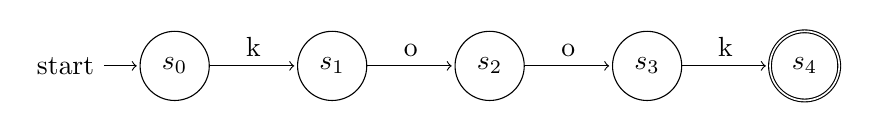
\begin{tikzpicture}[shorten >=1pt,node distance=2cm,on grid,auto]
    \node[state,initial] (s_0)                 {$s_0$};
    \node[state] (s_1)          [right=of s_0] {$s_1$};
    \node[state] (s_2)          [right=of s_1] {$s_2$};
    \node[state] (s_3)          [right=of s_2] {$s_3$};
    \node[state,accepting](s_4) [right=of s_3] {$s_4$};
    \path[->]
    (s_0) edge  node {k} (s_1)
    (s_1) edge  node {o} (s_2)
    (s_2) edge  node {o} (s_3)
    (s_3) edge  node {k} (s_4);
    % edge [loop below] node {1} ();
  \end{tikzpicture}
  \end{center}
\end{frame}


\begin{frame}
  \frametitle{Nondeterministic finite automaton}
  \begin{itemize}
  \item Introduced in 1959 \pause
  \item Recognize regular languages \pause
  \item Reading an input symbol is required for each state transition \pause
  \item Its transitions are not uniquely determined by its source
    state and input symbol \pause
  \end{itemize}
  And exist under many, many variations.
\end{frame}
% Difference between Thompson and Gluskov etc. automata
% http://www.cs.nyu.edu/~mohri/pub/glush.pdf

\begin{frame}
  \frametitle{Regexp? Automata?}
  Regexp = \ctexttt{ko*k}
  \par
  \par
  \begin{center}
  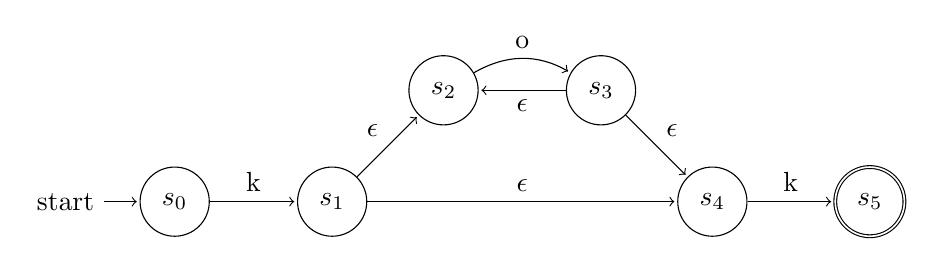
\begin{tikzpicture}[shorten >=1pt,node distance=2cm,on grid,auto]
    \node[state,initial] (s_0)                       {$s_0$};
    \node[state] (s_1)          [right=of s_0]       {$s_1$};
    \node[state] (s_2)          [above right=of s_1] {$s_2$};
    \node[state] (s_3)          [right=of s_2]       {$s_3$};
    \node[state] (s_4)          [below right=of s_3] {$s_4$};
    \node[state,accepting](s_5) [right=of s_4]       {$s_5$};
    \path[->]
    (s_0) edge node {k} (s_1)
    (s_1) edge node {$\epsilon$} (s_2)
    (s_3) edge node {$\epsilon$} (s_2)
    (s_2) edge [bend left] node {o} (s_3)
    (s_3) edge node {$\epsilon$} (s_4)
    (s_1) edge node {$\epsilon$} (s_4)
    (s_4) edge node {k} (s_5);
  \end{tikzpicture}
  \end{center}
\end{frame}


% ----- Animated example -------------------------------------------------------

% Step 0
\begin{frame}
  \frametitle{Another example}
  Regexp = \ctexttt{abab|abbb} \\
  Input = \ctexttt{$\rangle$abbb} \\
  \par
  \par
  \begin{center}
  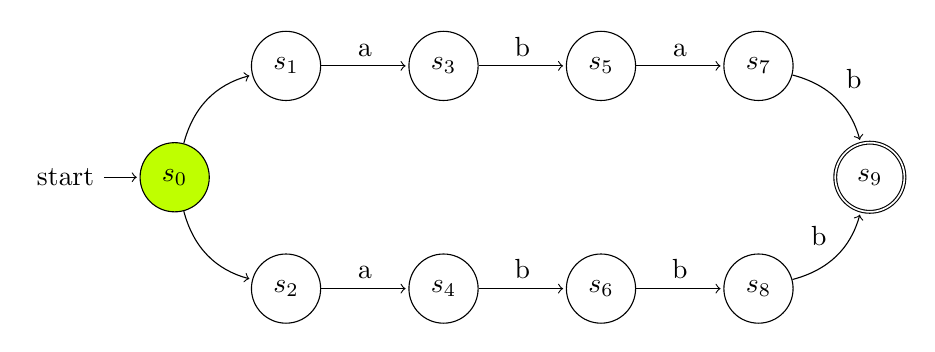
\begin{tikzpicture}[shorten >=1pt,node distance=2cm,on grid,auto]
    \node[state,initial] (s_0)  [fill=lime]   {$s_0$};
    \node[state] (s_1)          [above right=of s_0] {$s_1$};
    \node[state] (s_2)          [below right=of s_0] {$s_2$};
    \node[state] (s_3)          [right=of s_1]       {$s_3$};
    \node[state] (s_4)          [right=of s_2]       {$s_4$};
    \node[state] (s_5)          [right=of s_3]       {$s_5$};
    \node[state] (s_6)          [right=of s_4]       {$s_6$};
    \node[state] (s_7)          [right=of s_5]       {$s_7$};
    \node[state] (s_8)          [right=of s_6]       {$s_8$};
    \node[state,accepting](s_9) [below right=of s_7] {$s_9$};
    \path[->]
    (s_0) edge [bend left]  node {} (s_1)
    (s_0) edge [bend right] node {} (s_2)
    % top edges
    (s_1) edge node {a} (s_3)
    (s_3) edge node {b} (s_5)
    (s_5) edge node {a} (s_7)
    % bottom edges
    (s_2) edge node {a} (s_4)
    (s_4) edge node {b} (s_6)
    (s_6) edge node {b} (s_8)
    % final edges
    (s_7) edge [bend left]  node {b} (s_9)
    (s_8) edge [bend right] node {b} (s_9);
  \end{tikzpicture}
  \end{center}
\end{frame}

% Step 1
\begin{frame}
  \frametitle{Another example}
  Regexp = \ctexttt{abab|abbb} \\
  Input = \ctexttt{$\rangle$abbb}
  \par
  \par
  \begin{center}
  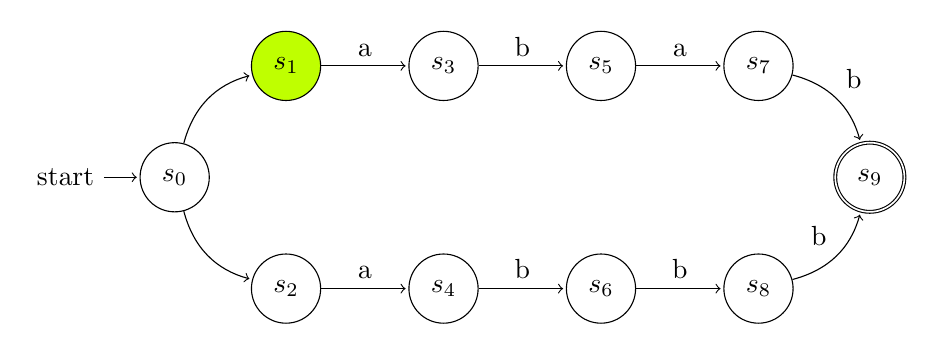
\begin{tikzpicture}[shorten >=1pt,node distance=2cm,on grid,auto]
    \node[state,initial] (s_0)                       {$s_0$};
    \node[state] (s_1)          [above right=of s_0] [fill=lime] {$s_1$};
    \node[state] (s_2)          [below right=of s_0] {$s_2$};
    \node[state] (s_3)          [right=of s_1]       {$s_3$};
    \node[state] (s_4)          [right=of s_2]       {$s_4$};
    \node[state] (s_5)          [right=of s_3]       {$s_5$};
    \node[state] (s_6)          [right=of s_4]       {$s_6$};
    \node[state] (s_7)          [right=of s_5]       {$s_7$};
    \node[state] (s_8)          [right=of s_6]       {$s_8$};
    \node[state,accepting](s_9) [below right=of s_7] {$s_9$};
    \path[->]
    (s_0) edge [bend left]  node {} (s_1)
    (s_0) edge [bend right] node {} (s_2)
    % top edges
    (s_1) edge node {a} (s_3)
    (s_3) edge node {b} (s_5)
    (s_5) edge node {a} (s_7)
    % bottom edges
    (s_2) edge node {a} (s_4)
    (s_4) edge node {b} (s_6)
    (s_6) edge node {b} (s_8)
    % final edges
    (s_7) edge [bend left]  node {b} (s_9)
    (s_8) edge [bend right] node {b} (s_9);
  \end{tikzpicture}
  \end{center}
\end{frame}

% Step 2
\begin{frame}
  \frametitle{Another example}
  Regexp = \ctexttt{abab|abbb} \\
  Input = \ctexttt{a$\rangle$bbb}
  \par
  \par
  \begin{center}
  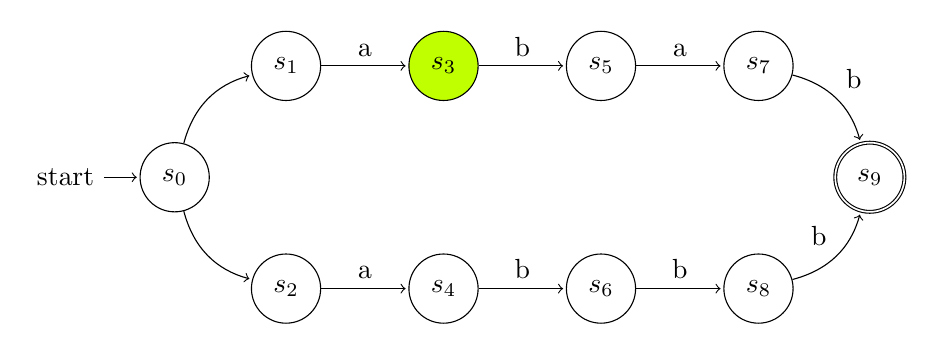
\begin{tikzpicture}[shorten >=1pt,node distance=2cm,on grid,auto]
    \node[state,initial] (s_0)                       {$s_0$};
    \node[state] (s_1)          [above right=of s_0] {$s_1$};
    \node[state] (s_2)          [below right=of s_0] {$s_2$};
    \node[state] (s_3)          [right=of s_1]       [fill=lime] {$s_3$};
    \node[state] (s_4)          [right=of s_2]       {$s_4$};
    \node[state] (s_5)          [right=of s_3]       {$s_5$};
    \node[state] (s_6)          [right=of s_4]       {$s_6$};
    \node[state] (s_7)          [right=of s_5]       {$s_7$};
    \node[state] (s_8)          [right=of s_6]       {$s_8$};
    \node[state,accepting](s_9) [below right=of s_7] {$s_9$};
    \path[->]
    (s_0) edge [bend left]  node {} (s_1)
    (s_0) edge [bend right] node {} (s_2)
    % top edges
    (s_1) edge node {a} (s_3)
    (s_3) edge node {b} (s_5)
    (s_5) edge node {a} (s_7)
    % bottom edges
    (s_2) edge node {a} (s_4)
    (s_4) edge node {b} (s_6)
    (s_6) edge node {b} (s_8)
    % final edges
    (s_7) edge [bend left]  node {b} (s_9)
    (s_8) edge [bend right] node {b} (s_9);
  \end{tikzpicture}
  \end{center}
\end{frame}

% Step 3
\begin{frame}
  \frametitle{Another example}
  Regexp = \ctexttt{abab|abbb} \\
  Input = \ctexttt{ab$\rangle$bb}
  \par
  \par
  \begin{center}
  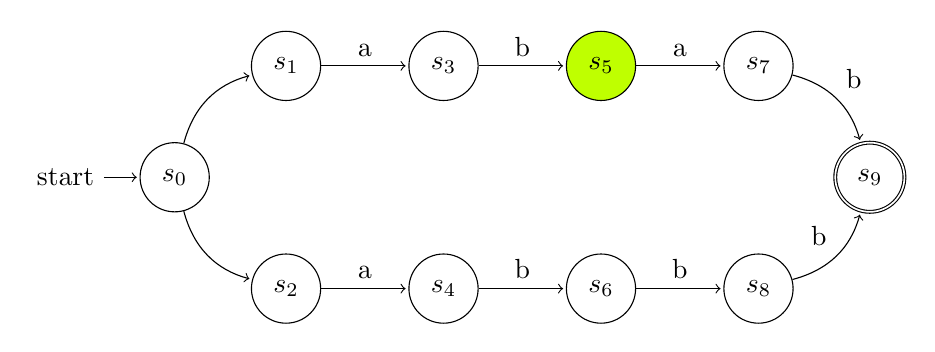
\begin{tikzpicture}[shorten >=1pt,node distance=2cm,on grid,auto]
    \node[state,initial] (s_0)                       {$s_0$};
    \node[state] (s_1)          [above right=of s_0] {$s_1$};
    \node[state] (s_2)          [below right=of s_0] {$s_2$};
    \node[state] (s_3)          [right=of s_1]       {$s_3$};
    \node[state] (s_4)          [right=of s_2]       {$s_4$};
    \node[state] (s_5)          [right=of s_3]       [fill=lime] {$s_5$};
    \node[state] (s_6)          [right=of s_4]       {$s_6$};
    \node[state] (s_7)          [right=of s_5]       {$s_7$};
    \node[state] (s_8)          [right=of s_6]       {$s_8$};
    \node[state,accepting](s_9) [below right=of s_7] {$s_9$};
    \path[->]
    (s_0) edge [bend left]  node {} (s_1)
    (s_0) edge [bend right] node {} (s_2)
    % top edges
    (s_1) edge node {a} (s_3)
    (s_3) edge node {b} (s_5)
    (s_5) edge node {a} (s_7)
    % bottom edges
    (s_2) edge node {a} (s_4)
    (s_4) edge node {b} (s_6)
    (s_6) edge node {b} (s_8)
    % final edges
    (s_7) edge [bend left]  node {b} (s_9)
    (s_8) edge [bend right] node {b} (s_9);
  \end{tikzpicture}
  \end{center}
\end{frame}

% Step 4
\begin{frame}
  \frametitle{Another example}
  Regexp = \ctexttt{abab|abbb} \\
  Input = \ctexttt{$\rangle$abbb}
  \par
  \par
  \begin{center}
  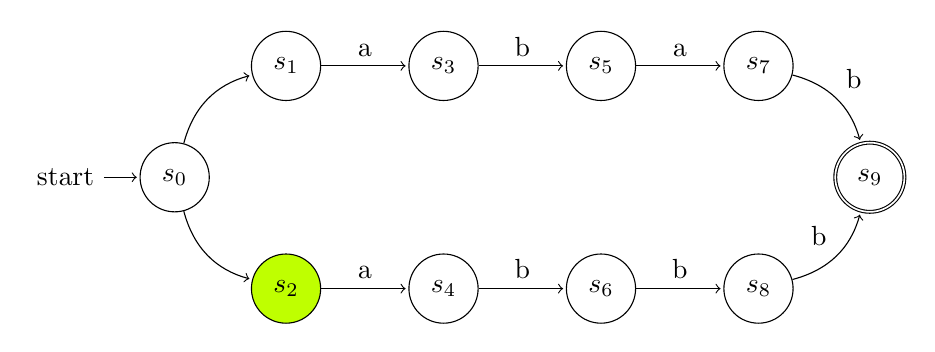
\begin{tikzpicture}[shorten >=1pt,node distance=2cm,on grid,auto]
    \node[state,initial] (s_0)                       {$s_0$};
    \node[state] (s_1)          [above right=of s_0] {$s_1$};
    \node[state] (s_2)          [below right=of s_0] [fill=lime] {$s_2$};
    \node[state] (s_3)          [right=of s_1]       {$s_3$};
    \node[state] (s_4)          [right=of s_2]       {$s_4$};
    \node[state] (s_5)          [right=of s_3]       {$s_5$};
    \node[state] (s_6)          [right=of s_4]       {$s_6$};
    \node[state] (s_7)          [right=of s_5]       {$s_7$};
    \node[state] (s_8)          [right=of s_6]       {$s_8$};
    \node[state,accepting](s_9) [below right=of s_7] {$s_9$};
    \path[->]
    (s_0) edge [bend left]  node {} (s_1)
    (s_0) edge [bend right] node {} (s_2)
    % top edges
    (s_1) edge node {a} (s_3)
    (s_3) edge node {b} (s_5)
    (s_5) edge node {a} (s_7)
    % bottom edges
    (s_2) edge node {a} (s_4)
    (s_4) edge node {b} (s_6)
    (s_6) edge node {b} (s_8)
    % final edges
    (s_7) edge [bend left]  node {b} (s_9)
    (s_8) edge [bend right] node {b} (s_9);
  \end{tikzpicture}
  \end{center}
\end{frame}

% Step 5
\begin{frame}
  \frametitle{Another example}
  Regexp = \ctexttt{abab|abbb} \\
  Input = \ctexttt{a$\rangle$bbb}
  \par
  \par
  \begin{center}
  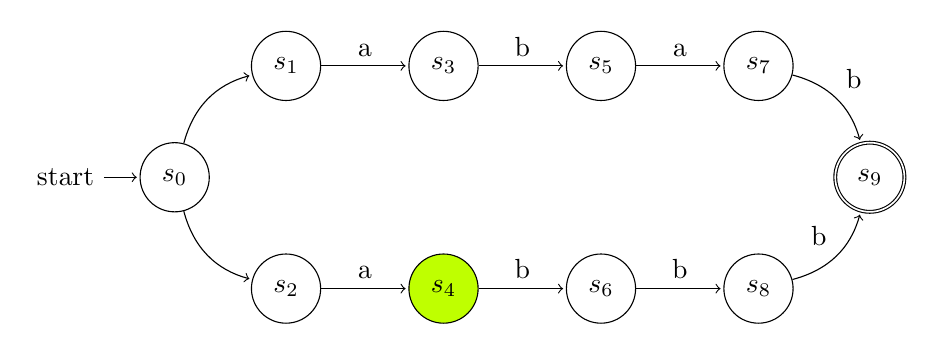
\begin{tikzpicture}[shorten >=1pt,node distance=2cm,on grid,auto]
    \node[state,initial] (s_0)                       {$s_0$};
    \node[state] (s_1)          [above right=of s_0] {$s_1$};
    \node[state] (s_2)          [below right=of s_0] {$s_2$};
    \node[state] (s_3)          [right=of s_1]       {$s_3$};
    \node[state] (s_4)          [right=of s_2]       [fill=lime] {$s_4$};
    \node[state] (s_5)          [right=of s_3]       {$s_5$};
    \node[state] (s_6)          [right=of s_4]       {$s_6$};
    \node[state] (s_7)          [right=of s_5]       {$s_7$};
    \node[state] (s_8)          [right=of s_6]       {$s_8$};
    \node[state,accepting](s_9) [below right=of s_7] {$s_9$};
    \path[->]
    (s_0) edge [bend left]  node {} (s_1)
    (s_0) edge [bend right] node {} (s_2)
    % top edges
    (s_1) edge node {a} (s_3)
    (s_3) edge node {b} (s_5)
    (s_5) edge node {a} (s_7)
    % bottom edges
    (s_2) edge node {a} (s_4)
    (s_4) edge node {b} (s_6)
    (s_6) edge node {b} (s_8)
    % final edges
    (s_7) edge [bend left]  node {b} (s_9)
    (s_8) edge [bend right] node {b} (s_9);
  \end{tikzpicture}
  \end{center}
\end{frame}

% Step 6
\begin{frame}
  \frametitle{Another example}
  Regexp = \ctexttt{abab|abbb} \\
  Input = \ctexttt{ab$\rangle$bb}
  \par
  \par
  \begin{center}
  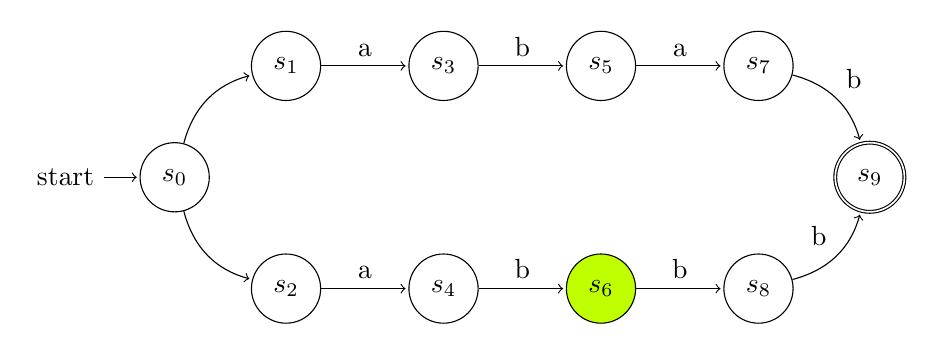
\begin{tikzpicture}[shorten >=1pt,node distance=2cm,on grid,auto]
    \node[state,initial] (s_0)                       {$s_0$};
    \node[state] (s_1)          [above right=of s_0] {$s_1$};
    \node[state] (s_2)          [below right=of s_0] {$s_2$};
    \node[state] (s_3)          [right=of s_1]       {$s_3$};
    \node[state] (s_4)          [right=of s_2]       {$s_4$};
    \node[state] (s_5)          [right=of s_3]       {$s_5$};
    \node[state] (s_6)          [right=of s_4]       [fill=lime] {$s_6$};
    \node[state] (s_7)          [right=of s_5]       {$s_7$};
    \node[state] (s_8)          [right=of s_6]       {$s_8$};
    \node[state,accepting](s_9) [below right=of s_7] {$s_9$};
    \path[->]
    (s_0) edge [bend left]  node {} (s_1)
    (s_0) edge [bend right] node {} (s_2)
    % top edges
    (s_1) edge node {a} (s_3)
    (s_3) edge node {b} (s_5)
    (s_5) edge node {a} (s_7)
    % bottom edges
    (s_2) edge node {a} (s_4)
    (s_4) edge node {b} (s_6)
    (s_6) edge node {b} (s_8)
    % final edges
    (s_7) edge [bend left]  node {b} (s_9)
    (s_8) edge [bend right] node {b} (s_9);
  \end{tikzpicture}
  \end{center}
\end{frame}

% Step 7
\begin{frame}
  \frametitle{Another example}
  Regexp = \ctexttt{abab|abbb} \\
  Input = \ctexttt{abb$\rangle$b}
  \par
  \par
  \begin{center}
  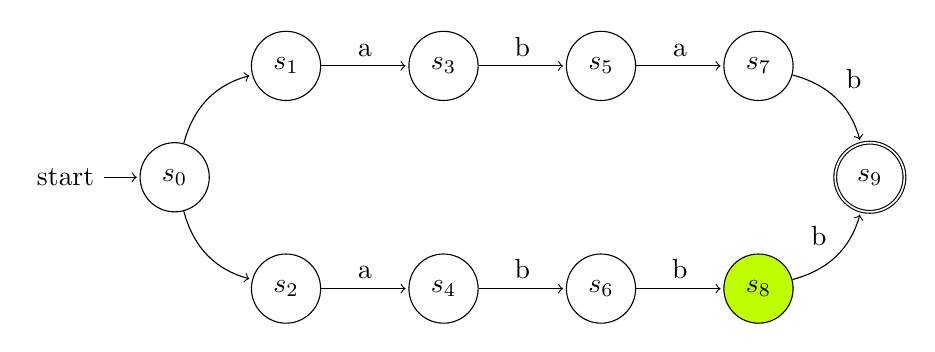
\begin{tikzpicture}[shorten >=1pt,node distance=2cm,on grid,auto]
    \node[state,initial] (s_0)                       {$s_0$};
    \node[state] (s_1)          [above right=of s_0] {$s_1$};
    \node[state] (s_2)          [below right=of s_0] {$s_2$};
    \node[state] (s_3)          [right=of s_1]       {$s_3$};
    \node[state] (s_4)          [right=of s_2]       {$s_4$};
    \node[state] (s_5)          [right=of s_3]       {$s_5$};
    \node[state] (s_6)          [right=of s_4]       {$s_6$};
    \node[state] (s_7)          [right=of s_5]       {$s_7$};
    \node[state] (s_8)          [right=of s_6]       [fill=lime] {$s_8$};
    \node[state,accepting](s_9) [below right=of s_7] {$s_9$};
    \path[->]
    (s_0) edge [bend left]  node {} (s_1)
    (s_0) edge [bend right] node {} (s_2)
    % top edges
    (s_1) edge node {a} (s_3)
    (s_3) edge node {b} (s_5)
    (s_5) edge node {a} (s_7)
    % bottom edges
    (s_2) edge node {a} (s_4)
    (s_4) edge node {b} (s_6)
    (s_6) edge node {b} (s_8)
    % final edges
    (s_7) edge [bend left]  node {b} (s_9)
    (s_8) edge [bend right] node {b} (s_9);
  \end{tikzpicture}
  \end{center}
\end{frame}

% Step 8
\begin{frame}
  \frametitle{Another example}
  Regexp = \ctexttt{abab|abbb} \\
  Input = \ctexttt{abbb$\rangle$}
  \par
  \par
  \begin{center}
  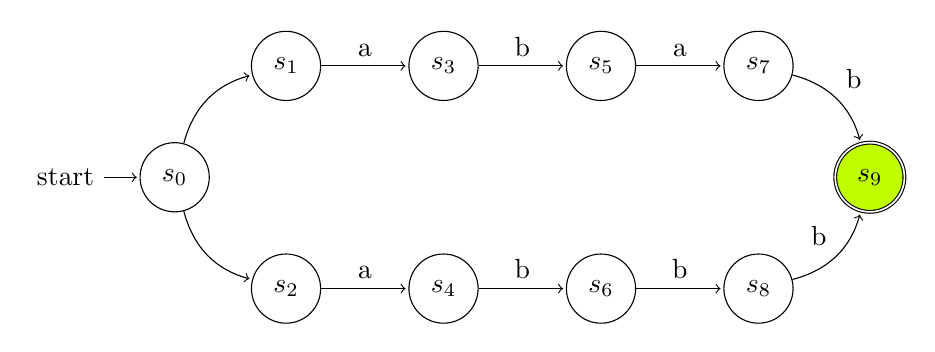
\begin{tikzpicture}[shorten >=1pt,node distance=2cm,on grid,auto]
    \node[state,initial] (s_0)                       {$s_0$};
    \node[state] (s_1)          [above right=of s_0] {$s_1$};
    \node[state] (s_2)          [below right=of s_0] {$s_2$};
    \node[state] (s_3)          [right=of s_1]       {$s_3$};
    \node[state] (s_4)          [right=of s_2]       {$s_4$};
    \node[state] (s_5)          [right=of s_3]       {$s_5$};
    \node[state] (s_6)          [right=of s_4]       {$s_6$};
    \node[state] (s_7)          [right=of s_5]       {$s_7$};
    \node[state] (s_8)          [right=of s_6]       {$s_8$};
    \node[state,accepting](s_9) [below right=of s_7] [fill=lime] {$s_9$};
    \path[->]
    (s_0) edge [bend left]  node {} (s_1)
    (s_0) edge [bend right] node {} (s_2)
    % top edges
    (s_1) edge node {a} (s_3)
    (s_3) edge node {b} (s_5)
    (s_5) edge node {a} (s_7)
    % bottom edges
    (s_2) edge node {a} (s_4)
    (s_4) edge node {b} (s_6)
    (s_6) edge node {b} (s_8)
    % final edges
    (s_7) edge [bend left]  node {b} (s_9)
    (s_8) edge [bend right] node {b} (s_9);
  \end{tikzpicture}
  \end{center}
\end{frame}

% ----- End of Animated example -------------------------------------------------

\begin{frame}
  \frametitle{Problem}
  \begin{alertblock}{Problem}
    Backtracking!
  \end{alertblock}
  This is what happened with \ctexttt{(a?){26}(a){26}}.
  (At least) 2 alternatives:
  \begin{itemize}
  \item Thompson's NFA
  \item DFA (Deterministic Finite Automaton)
  \end{itemize}
\end{frame}


\begin{frame}
  \frametitle{Alternative 1: Thompson's NFA}
  \begin{itemize}
  \item Optimized by Ken Thompson, (Bell Telphone Labs Inc.), in a
    1968 CACM paper
  \item Allows several possible states at the same moment
  \end{itemize}
\end{frame}


\begin{frame}
  \frametitle{Ken Thompson}
  \begin{columns}[T]
    \begin{column}{.3\textwidth}
      \begin{center}
        \includegraphics[width=100px]{images/ken-thompson.png}
      \end{center}
    \end{column}
    \begin{column}{.7\textwidth}
      \begin{itemize}
        \item American computer scientist (1943) \pause
        \item Designed and implemented the original Unix operating
          system \pause
        \item Co-invented the Go programming language \pause
        \item Turing Award (for \textit{backdoor attack})
      \end{itemize}
    \end{column}
  \end{columns}
\end{frame}


% ----- Start of Animated example -----------------------------------------------

% Step 0
\begin{frame}
  \frametitle{Thompson's NFA example}
  Regexp = \ctexttt{abab|abbb} \\
  Input = \ctexttt{$\rangle$abbb}
  \par
  \par
  \begin{center}
  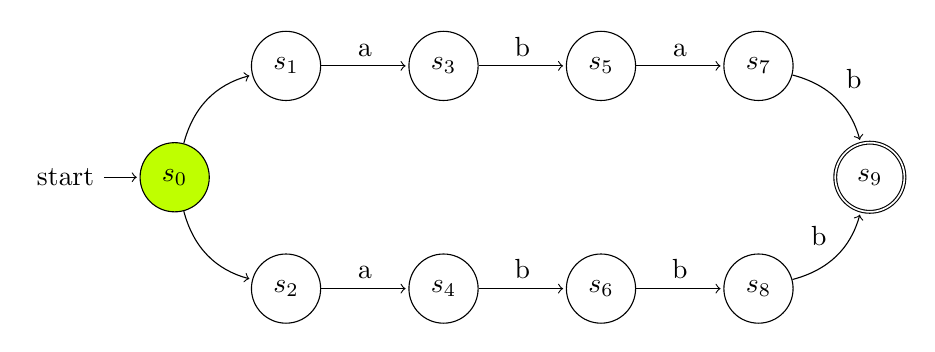
\begin{tikzpicture}[shorten >=1pt,node distance=2cm,on grid,auto]
    \node[state,initial] (s_0)                       [fill=lime] {$s_0$};
    \node[state] (s_1)          [above right=of s_0] {$s_1$};
    \node[state] (s_2)          [below right=of s_0] {$s_2$};
    \node[state] (s_3)          [right=of s_1]       {$s_3$};
    \node[state] (s_4)          [right=of s_2]       {$s_4$};
    \node[state] (s_5)          [right=of s_3]       {$s_5$};
    \node[state] (s_6)          [right=of s_4]       {$s_6$};
    \node[state] (s_7)          [right=of s_5]       {$s_7$};
    \node[state] (s_8)          [right=of s_6]       {$s_8$};
    \node[state,accepting](s_9) [below right=of s_7] {$s_9$};
    \path[->]
    (s_0) edge [bend left]  node {} (s_1)
    (s_0) edge [bend right] node {} (s_2)
    % top edges
    (s_1) edge node {a} (s_3)
    (s_3) edge node {b} (s_5)
    (s_5) edge node {a} (s_7)
    % bottom edges
    (s_2) edge node {a} (s_4)
    (s_4) edge node {b} (s_6)
    (s_6) edge node {b} (s_8)
    % final edges
    (s_7) edge [bend left]  node {b} (s_9)
    (s_8) edge [bend right] node {b} (s_9);
  \end{tikzpicture}
  \end{center}
\end{frame}

% Step 1
\begin{frame}
  \frametitle{Thompson's NFA example}
  Regexp = \ctexttt{abab|abbb} \\
  Input = \ctexttt{$\rangle$abbb}
  \par
  \par
  \begin{center}
  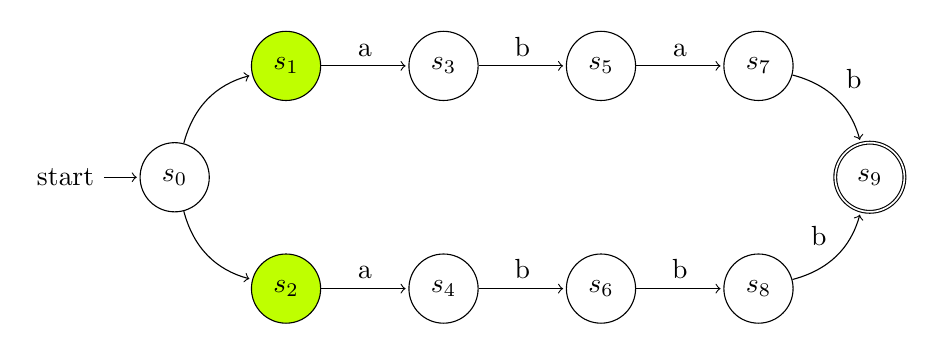
\begin{tikzpicture}[shorten >=1pt,node distance=2cm,on grid,auto]
    \node[state,initial] (s_0)                       {$s_0$};
    \node[state] (s_1)          [above right=of s_0] [fill=lime] {$s_1$};
    \node[state] (s_2)          [below right=of s_0] [fill=lime] {$s_2$};
    \node[state] (s_3)          [right=of s_1]       {$s_3$};
    \node[state] (s_4)          [right=of s_2]       {$s_4$};
    \node[state] (s_5)          [right=of s_3]       {$s_5$};
    \node[state] (s_6)          [right=of s_4]       {$s_6$};
    \node[state] (s_7)          [right=of s_5]       {$s_7$};
    \node[state] (s_8)          [right=of s_6]       {$s_8$};
    \node[state,accepting](s_9) [below right=of s_7] {$s_9$};
    \path[->]
    (s_0) edge [bend left]  node {} (s_1)
    (s_0) edge [bend right] node {} (s_2)
    % top edges
    (s_1) edge node {a} (s_3)
    (s_3) edge node {b} (s_5)
    (s_5) edge node {a} (s_7)
    % bottom edges
    (s_2) edge node {a} (s_4)
    (s_4) edge node {b} (s_6)
    (s_6) edge node {b} (s_8)
    % final edges
    (s_7) edge [bend left]  node {b} (s_9)
    (s_8) edge [bend right] node {b} (s_9);
  \end{tikzpicture}
  \end{center}
\end{frame}


% Step 2
\begin{frame}
  \frametitle{Thompson's NFA example}
  Regexp = \ctexttt{abab|abbb} \\
  Input = \ctexttt{a$\rangle$bbb}
  \par
  \par
  \begin{center}
  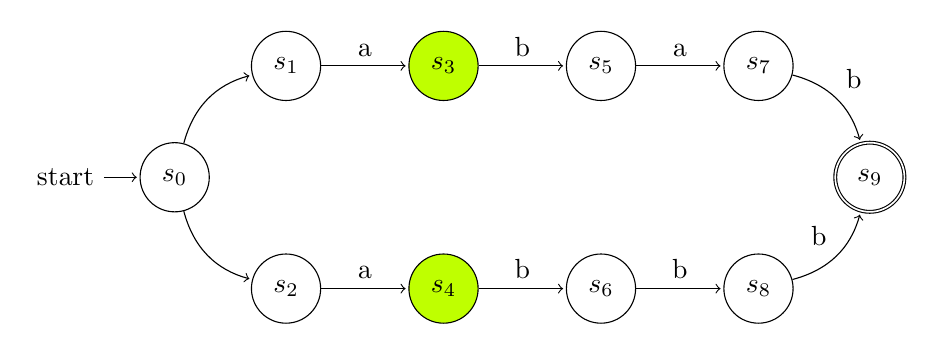
\begin{tikzpicture}[shorten >=1pt,node distance=2cm,on grid,auto]
    \node[state,initial] (s_0)                       {$s_0$};
    \node[state] (s_1)          [above right=of s_0] {$s_1$};
    \node[state] (s_2)          [below right=of s_0] {$s_2$};
    \node[state] (s_3)          [right=of s_1]       [fill=lime] {$s_3$};
    \node[state] (s_4)          [right=of s_2]       [fill=lime] {$s_4$};
    \node[state] (s_5)          [right=of s_3]       {$s_5$};
    \node[state] (s_6)          [right=of s_4]       {$s_6$};
    \node[state] (s_7)          [right=of s_5]       {$s_7$};
    \node[state] (s_8)          [right=of s_6]       {$s_8$};
    \node[state,accepting](s_9) [below right=of s_7] {$s_9$};
    \path[->]
    (s_0) edge [bend left]  node {} (s_1)
    (s_0) edge [bend right] node {} (s_2)
    % top edges
    (s_1) edge node {a} (s_3)
    (s_3) edge node {b} (s_5)
    (s_5) edge node {a} (s_7)
    % bottom edges
    (s_2) edge node {a} (s_4)
    (s_4) edge node {b} (s_6)
    (s_6) edge node {b} (s_8)
    % final edges
    (s_7) edge [bend left]  node {b} (s_9)
    (s_8) edge [bend right] node {b} (s_9);
  \end{tikzpicture}
  \end{center}
\end{frame}


% Step 3
\begin{frame}
  \frametitle{Thompson's NFA example}
  Regexp = \ctexttt{abab|abbb} \\
  Input = \ctexttt{ab$\rangle$bb}
  \par
  \par
  \begin{center}
  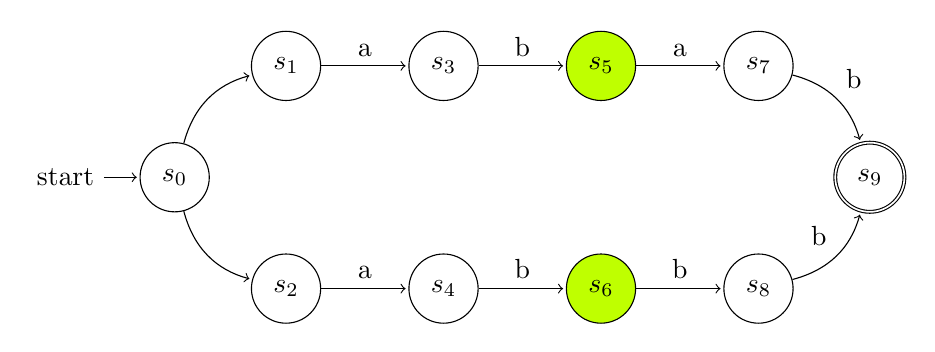
\begin{tikzpicture}[shorten >=1pt,node distance=2cm,on grid,auto]
    \node[state,initial] (s_0)                       {$s_0$};
    \node[state] (s_1)          [above right=of s_0] {$s_1$};
    \node[state] (s_2)          [below right=of s_0] {$s_2$};
    \node[state] (s_3)          [right=of s_1]       {$s_3$};
    \node[state] (s_4)          [right=of s_2]       {$s_4$};
    \node[state] (s_5)          [right=of s_3]       [fill=lime] {$s_5$};
    \node[state] (s_6)          [right=of s_4]       [fill=lime] {$s_6$};
    \node[state] (s_7)          [right=of s_5]       {$s_7$};
    \node[state] (s_8)          [right=of s_6]       {$s_8$};
    \node[state,accepting](s_9) [below right=of s_7] {$s_9$};
    \path[->]
    (s_0) edge [bend left]  node {} (s_1)
    (s_0) edge [bend right] node {} (s_2)
    % top edges
    (s_1) edge node {a} (s_3)
    (s_3) edge node {b} (s_5)
    (s_5) edge node {a} (s_7)
    % bottom edges
    (s_2) edge node {a} (s_4)
    (s_4) edge node {b} (s_6)
    (s_6) edge node {b} (s_8)
    % final edges
    (s_7) edge [bend left]  node {b} (s_9)
    (s_8) edge [bend right] node {b} (s_9);
  \end{tikzpicture}
  \end{center}
\end{frame}


% Step 4
\begin{frame}
  \frametitle{Thompson's NFA example}
  Regexp = \ctexttt{abab|abbb} \\
  Input = \ctexttt{abb$\rangle$b}
  \par
  \par
  \begin{center}
  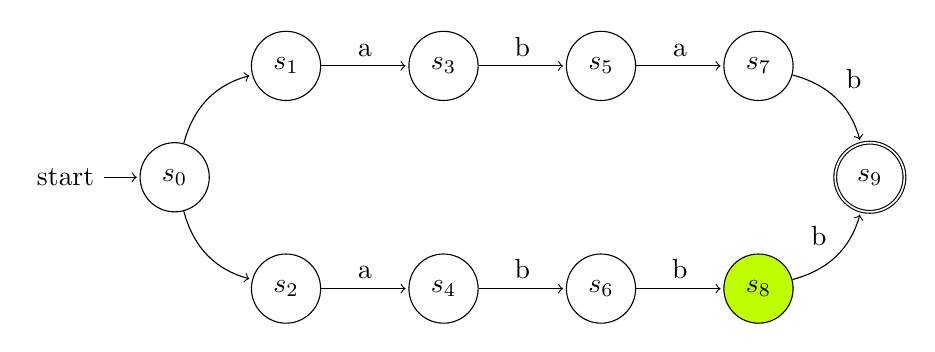
\begin{tikzpicture}[shorten >=1pt,node distance=2cm,on grid,auto]
    \node[state,initial] (s_0)                       {$s_0$};
    \node[state] (s_1)          [above right=of s_0] {$s_1$};
    \node[state] (s_2)          [below right=of s_0] {$s_2$};
    \node[state] (s_3)          [right=of s_1]       {$s_3$};
    \node[state] (s_4)          [right=of s_2]       {$s_4$};
    \node[state] (s_5)          [right=of s_3]       {$s_5$};
    \node[state] (s_6)          [right=of s_4]       {$s_6$};
    \node[state] (s_7)          [right=of s_5]       {$s_7$};
    \node[state] (s_8)          [right=of s_6]       [fill=lime] {$s_8$};
    \node[state,accepting](s_9) [below right=of s_7] {$s_9$};
    \path[->]
    (s_0) edge [bend left]  node {} (s_1)
    (s_0) edge [bend right] node {} (s_2)
    % top edges
    (s_1) edge node {a} (s_3)
    (s_3) edge node {b} (s_5)
    (s_5) edge node {a} (s_7)
    % bottom edges
    (s_2) edge node {a} (s_4)
    (s_4) edge node {b} (s_6)
    (s_6) edge node {b} (s_8)
    % final edges
    (s_7) edge [bend left]  node {b} (s_9)
    (s_8) edge [bend right] node {b} (s_9);
  \end{tikzpicture}
  \end{center}
\end{frame}


% Step 5
\begin{frame}
  \frametitle{Thompson's NFA example}
  Regexp = \ctexttt{abab|abbb} \\
  Input = \ctexttt{abbb$\rangle$}
  \par
  \par
  \begin{center}
  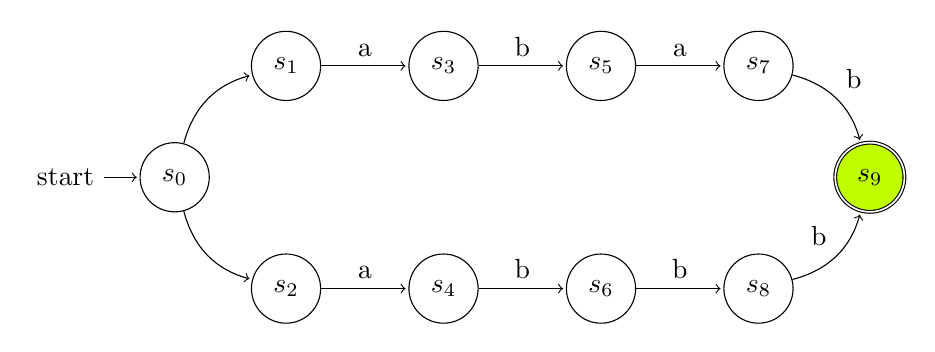
\begin{tikzpicture}[shorten >=1pt,node distance=2cm,on grid,auto]
    \node[state,initial] (s_0)                       {$s_0$};
    \node[state] (s_1)          [above right=of s_0] {$s_1$};
    \node[state] (s_2)          [below right=of s_0] {$s_2$};
    \node[state] (s_3)          [right=of s_1]       {$s_3$};
    \node[state] (s_4)          [right=of s_2]       {$s_4$};
    \node[state] (s_5)          [right=of s_3]       {$s_5$};
    \node[state] (s_6)          [right=of s_4]       {$s_6$};
    \node[state] (s_7)          [right=of s_5]       {$s_7$};
    \node[state] (s_8)          [right=of s_6]       {$s_8$};
    \node[state,accepting](s_9) [below right=of s_7] [fill=lime] {$s_9$};
    \path[->]
    (s_0) edge [bend left]  node {} (s_1)
    (s_0) edge [bend right] node {} (s_2)
    % top edges
    (s_1) edge node {a} (s_3)
    (s_3) edge node {b} (s_5)
    (s_5) edge node {a} (s_7)
    % bottom edges
    (s_2) edge node {a} (s_4)
    (s_4) edge node {b} (s_6)
    (s_6) edge node {b} (s_8)
    % final edges
    (s_7) edge [bend left]  node {b} (s_9)
    (s_8) edge [bend right] node {b} (s_9);
  \end{tikzpicture}
  \end{center}
\end{frame}


% ----- End of Animated example -------------------------------------------------


\begin{frame}
  \begin{figure}
    \includegraphics[width=350px]{images/grep1p.png}
    \caption{\url{https://swtch.com/~rsc/regexp/regexp1.html}}
  \end{figure}
\end{frame}


\begin{frame}
  \frametitle{Alternative 2: DFA}
  \begin{block}{Property}
    Each of its transitions is \textbf{uniquely} determined by its source state and
    input symbol
  \end{block}
  \begin{block}{Theorem}
    Every NFA as an equivalent DFA
    [\href{https://courses.engr.illinois.edu/cs373/fa2013/Lectures/lec05.pdf}{proof}]
  \end{block}
\end{frame}


% ----- Start of Animated example -----------------------------------------------

% Step 0
\begin{frame}
  \frametitle{DFA example}
  Regexp = \ctexttt{abab|abbb} \\
  Input = \ctexttt{$\rangle$abbb}
  \par
  \par
  \begin{center}
  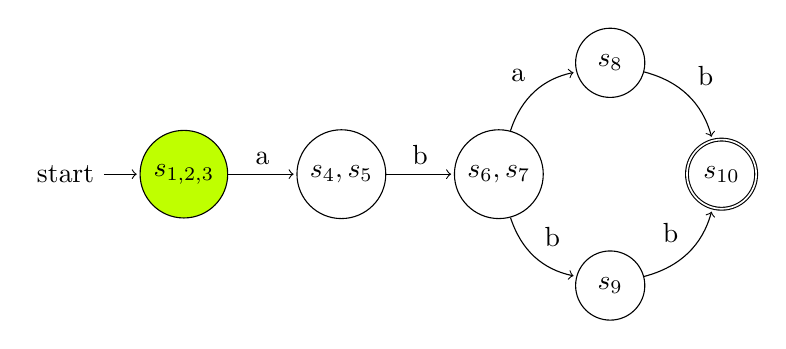
\begin{tikzpicture}[shorten >=1pt,node distance=2cm,on grid,auto]
    \node[state,initial] (s_123)                 [fill=lime] {$s_{1,2,3}$};
    \node[state] (s_245)        [right=of s_123]       {$s_4, s_5$};
    \node[state] (s_67)         [right=of s_245]       {$s_6, s_7$};
    \node[state] (s_8)          [above right=of s_67]  {$s_8$};
    \node[state] (s_9)          [below right=of s_67]  {$s_9$};
    \node[state,accepting] (s_10)   [below right=of s_8]   {$s_{10}$};
    \path[->]
    (s_123) edge node {a} (s_245)
    (s_245) edge node {b} (s_67)
    (s_67)  edge [bend left] node {a} (s_8)
    (s_67)  edge [bend right] node {b} (s_9)
    (s_8)   edge [bend left] node {b} (s_10)
    (s_9)   edge [bend right] node {b} (s_10);
  \end{tikzpicture}
  \end{center}
\end{frame}


% Step 1
\begin{frame}
  \frametitle{DFA example}
  Regexp = \ctexttt{abab|abbb} \\
  Input = \ctexttt{a$\rangle$bbb}
  \par
  \par
  \begin{center}
  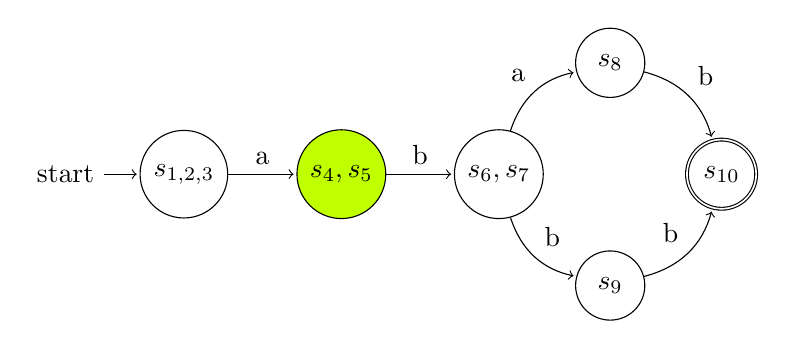
\begin{tikzpicture}[shorten >=1pt,node distance=2cm,on grid,auto]
    \node[state,initial] (s_123)                       {$s_{1,2,3}$};
    \node[state] (s_245)        [right=of s_123] [fill=lime] {$s_4, s_5$};
    \node[state] (s_67)         [right=of s_245]       {$s_6, s_7$};
    \node[state] (s_8)          [above right=of s_67]  {$s_8$};
    \node[state] (s_9)          [below right=of s_67]  {$s_9$};
    \node[state,accepting] (s_10)   [below right=of s_8]   {$s_{10}$};
    \path[->]
    (s_123) edge node {a} (s_245)
    (s_245) edge node {b} (s_67)
    (s_67)  edge [bend left] node {a} (s_8)
    (s_67)  edge [bend right] node {b} (s_9)
    (s_8)   edge [bend left] node {b} (s_10)
    (s_9)   edge [bend right] node {b} (s_10);
  \end{tikzpicture}
  \end{center}
\end{frame}


% Step 2
\begin{frame}
  \frametitle{DFA example}
  Regexp = \ctexttt{abab|abbb} \\
  Input = \ctexttt{ab$\rangle$bb}
  \par
  \par
  \begin{center}
  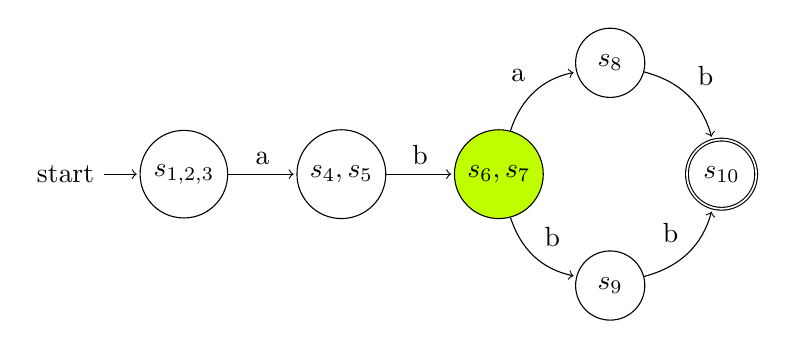
\begin{tikzpicture}[shorten >=1pt,node distance=2cm,on grid,auto]
    \node[state,initial] (s_123)                       {$s_{1,2,3}$};
    \node[state] (s_245)        [right=of s_123]       {$s_4, s_5$};
    \node[state] (s_67)         [right=of s_245] [fill=lime] {$s_6, s_7$};
    \node[state] (s_8)          [above right=of s_67]  {$s_8$};
    \node[state] (s_9)          [below right=of s_67]  {$s_9$};
    \node[state,accepting] (s_10)   [below right=of s_8]   {$s_{10}$};
    \path[->]
    (s_123) edge node {a} (s_245)
    (s_245) edge node {b} (s_67)
    (s_67)  edge [bend left] node {a} (s_8)
    (s_67)  edge [bend right] node {b} (s_9)
    (s_8)   edge [bend left] node {b} (s_10)
    (s_9)   edge [bend right] node {b} (s_10);
  \end{tikzpicture}
  \end{center}
\end{frame}


% Step 3
\begin{frame}
  \frametitle{DFA example}
  Regexp = \ctexttt{abab|abbb} \\
  Input = \ctexttt{abb$\rangle$b}
  \par
  \par
  \begin{center}
  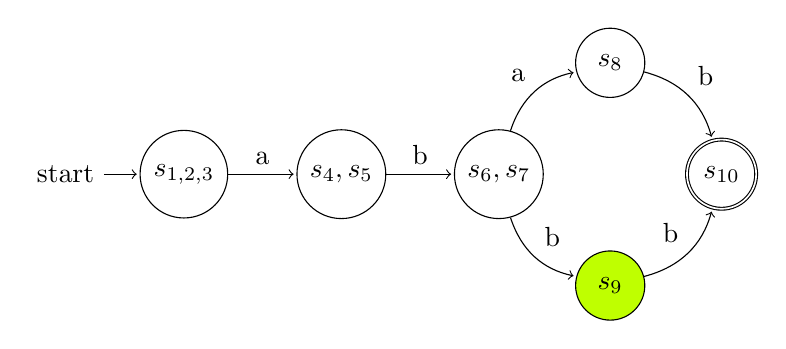
\begin{tikzpicture}[shorten >=1pt,node distance=2cm,on grid,auto]
    \node[state,initial] (s_123)                       {$s_{1,2,3}$};
    \node[state] (s_245)        [right=of s_123]       {$s_4, s_5$};
    \node[state] (s_67)         [right=of s_245]       {$s_6, s_7$};
    \node[state] (s_8)          [above right=of s_67]  {$s_8$};
    \node[state] (s_9)          [below right=of s_67] [fill=lime] {$s_9$};
    \node[state,accepting] (s_10)   [below right=of s_8]   {$s_{10}$};
    \path[->]
    (s_123) edge node {a} (s_245)
    (s_245) edge node {b} (s_67)
    (s_67)  edge [bend left] node {a} (s_8)
    (s_67)  edge [bend right] node {b} (s_9)
    (s_8)   edge [bend left] node {b} (s_10)
    (s_9)   edge [bend right] node {b} (s_10);
  \end{tikzpicture}
  \end{center}
\end{frame}


% Step 4
\begin{frame}
  \frametitle{DFA example}
  Regexp = \ctexttt{abab|abbb} \\
  Input = \ctexttt{abbb$\rangle$}
  \par
  \par
  \begin{center}
  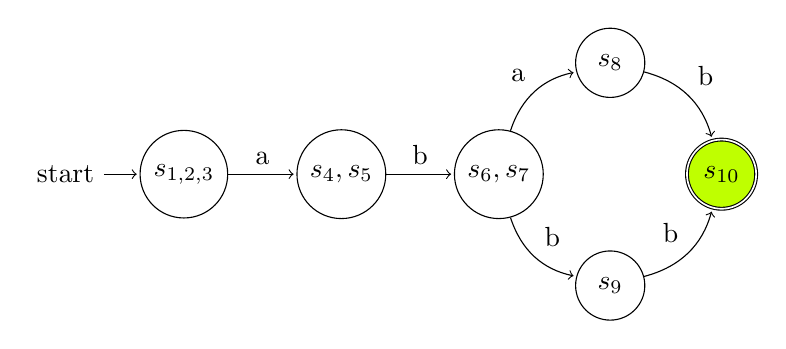
\begin{tikzpicture}[shorten >=1pt,node distance=2cm,on grid,auto]
    \node[state,initial] (s_123)                       {$s_{1,2,3}$};
    \node[state] (s_245)        [right=of s_123]       {$s_4, s_5$};
    \node[state] (s_67)         [right=of s_245]       {$s_6, s_7$};
    \node[state] (s_8)          [above right=of s_67]  {$s_8$};
    \node[state] (s_9)          [below right=of s_67]  {$s_9$};
    \node[state,accepting] (s_10)   [below right=of s_8] [fill=lime] {$s_{10}$};
    \path[->]
    (s_123) edge node {a} (s_245)
    (s_245) edge node {b} (s_67)
    (s_67)  edge [bend left] node {a} (s_8)
    (s_67)  edge [bend right] node {b} (s_9)
    (s_8)   edge [bend left] node {b} (s_10)
    (s_9)   edge [bend right] node {b} (s_10);
  \end{tikzpicture}
  \end{center}
\end{frame}


% ----- End of Animated example -------------------------------------------------


\begin{frame}
  \frametitle{Mistery from History}
  \begin{quotation}
    Why don't everyone use Thompson's NFA or DFA???
  \end{quotation}
\end{frame}


\begin{frame}
  \frametitle{You're not alone}
  \begin{itemize}
  \item Java's \ctexttt{java.util.regex} uses backtracking too, so does PHP
    (PCRE library).
  \item Tcl, Awk, GNU Awk and GNU grep all use... DFA's!
  \item Google RE2 offers a C++ implementation (+ wrappers)
  \end{itemize}
\end{frame}


\begin{frame}
  \frametitle{PCRE vs Google RE2}
  \begin{center}
    \begin{figure}
      \includegraphics[width=230px]{images/pcre-vs-re2.png}
      \caption{Numbers from \url{http://sljit.sourceforge.net/regex\_perf.html}}
    \end{figure}
  \end{center}
\end{frame}


\begin{frame}
  \frametitle{Limitations}
  \begin{itemize}
    \item Backreferences (\textit{e.g.} \ctexttt{
        <(.+)>(.*)</(\textbackslash1)>} to identify a closing XML tag)
    \item Space consumption of DFA can be way higher: \\ NFA: $O(n)$,
      DFA: $O(2^{n}$), $n$ is for regexp's length
  \end{itemize}
\end{frame}


\begin{frame}
  \frametitle{Conclusion}
  \begin{itemize}
    \item Be careful when using regexes
    \item Think about underlying engine
    \item Think about worst case usage (user's inputs...)
    \item Think about \ctexttt{strstr()}
  \end{itemize}
\end{frame}


\begin{frame}
  \frametitle{Bibliography}
  \begin{itemize}
  \item \url{https://en.wikipedia.org/wiki/Regular\_language}
  \item \url{https://en.wikipedia.org/wiki/Chomsky\_hierarchy}
  \item \url{https://en.wikipedia.org/wiki/Stephen\_Cole\_Kleene}
  \item \url{http://www.cs.ucr.edu/~jiang/cs215/tao-new.pdf}
  \item \url{https://www.debuggex.com/}
  \item \url{http://www.borntosegfault.com/2013/03/regexp-think-dfa.html}
  \item \url{http://sljit.sourceforge.net/regex\_perf.html}
  \item \url{https://en.wikipedia.org/wiki/Thompson's\_construction}
  \end{itemize}
\end{frame}


\begin{frame}
  \frametitle{\sout{Trolls} Discussions}
  \begin{itemize}
  \item \url{http://arstechnica.com/civis/viewtopic.php?f=20\&t=1195549}
  \item \url{http://www.perlmonks.org/?node\_id=597262}
  \end{itemize}
\end{frame}

\begin{frame}
  \frametitle{Illustrations}
  \begin{itemize}
  \item \url{https://en.wikipedia.org/wiki/File:Chomsky-hierarchy.svg}
  \item \url{https://en.wikipedia.org/wiki/File:Kleene.jpg}
  \item \url{https://en.wikipedia.org/wiki/File:Noam\_Chomsky\_portrait\_2015.jpg}
  \end{itemize}
\end{frame}

\end{document}
